\chapter{神经符号框架的架构设计与实现}
\section{引言}
本章对神经符号框架的架构进行详细的介绍,包括流水线总体架构、视觉场景理解、语义解析、知识蒸馏、迭代反馈和规则修正、ASP推理等模块的设计和实现。
框架的目标如下:
\begin{enumerate}[label=(\arabic*),itemsep=0pt,parsep=0pt]
\item 增强VQA系统在复杂空间关系推理方面的能力。
\item 使用Dspy来完成对LLM的提示、优化,以降低神经符号方法的开发难度,并增强其可扩展性。
\end{enumerate}
\section{框架总体架构}
框架的总体架构如图所示。

LLM在整个框架中的作用有以下两点:
\begin{enumerate}[label=(\arabic*),itemsep=0pt,parsep=0pt]
    \item 在语义解析模块中,对自然语言问题进行语义解析,将问题以ASP程序的形式表示出来。
    \item 在迭代反馈模块中,对ASP表示进行多次迭代优化,其中包括:
添加规则,对规则进行一致性检查以及整合错误信息的反馈。
\end{enumerate}

本文在语义解析模块和迭代反馈模块中,分别采用不同的LLM,各自进行微调,以更好地满足不同任务的需求。
\section{视觉场景理解}
视觉场景理解是整个流水线的重要任务之一,其目标是从输入图像中提取结构化的信息,包括物体的属性(形状、颜色、大小等)、位置以及物体之间的空间关系。
这些信息随后以ASP程序来表示,为使用ASP求解器进行推理提供基础。本文选择使用GLIP模型来完成目标检测任务,以实现高效且准确的目标检测和定位。
下面本文
\subsection{目标检测}
目标检测是视觉场景理解的最基础的任务,其目标是从图像中识别出所有相关物体,并标注其边界框、类别和属性。本文选择GLIP模型作为目标检测的实现工具,原因在于
其独特的语言-视觉预训练特性。基于大规模的图文对数据,GLIP进行大量预训练,能够根据自然语言描述(如“红色立方体”)直接定位图像中的对应物体。
这种能力特别适合VQA任务,使问题中的语言信息与图像内容高效对齐成为可能。

具体到实现中,本文首先对输入图像进行预处理,将其调整为GLIP模型的输入分辨率(例如,800×1333像素)。
随后,构造一组文本提示,以覆盖图像中可能出现的物体。考虑到本文第三章构造的数据集,本文使用以下短语集合:
\begin{enumerate}[label=(\arabic*),itemsep=0pt,parsep=0pt]
    \item “大物体”、“小物体”等,描述物体的大小。
    \item “红色立方体”、“蓝色球体”、“绿色圆柱体”等,涵盖所有颜色和形状的组合。
\end{enumerate}
GLIP接收这些文本提示和图像作为输入,输出每个物体的边界框及其对应的类别标签。例如,对于一张包含“红色立方体”和“蓝色球体”的图像,GLIP的输出可能如下:
\begin{enumerate}
    \item 物体1:类别=“红色立方体”,边界框=($x_1$, $y_1$, $x_2$, $y_2$)。
    \item 物体2:类别=“蓝色球体”,边界框=($x_3$, $y_3$, $x_4$, $y_4$)。
\end{enumerate}

为了进一步提取物体的属性(如颜色、形状和大小),本文对GLIP的类别标签进行解析,将其分解为单独的属性值。例如,“红色立方体”被分解成color=red、shape=cube。
此外,通过边界框的面积(即$(x_2-x_1)\times (y_2-y_1)$),本文进一步推断物体的大小属性,设定阈值以区分“大”和“小”物体。
\subsection{空间位置提取}
在完成目标检测后,需要确定每个物体的空间位置,以便为空间关系推理提供依据。
GLIP提供的边界框信息为位置提取提供了基础。本文使用以下方法计算物体的空间位置:
\begin{enumerate}[label=(\arabic*),itemsep=0pt,parsep=0pt]
    \item 中心点坐标:对于每个物体,计算其边界框的中心点坐标($x_c, y_c$),其中:
    $$x_c = \frac{x_1 + x_2}{2}, y_c \frac{y_1+y_2}{2}$$
    该坐标表示物体在二维图像中的位置。
    \item 深度信息:通过图像的深度信息进一步推断物体的三维位置($x$,$y$,$z$)。由于
本文生成的数据集时使用的为Blender渲染引擎,故可直接从渲染引擎中获取深度信息。
\end{enumerate}

最终,每个物体的位置信息被表示为ASP事实,例如:position(obj1, x1c, y1c, z1) 表示物体1的中心点位置。

\subsection{空间关系提取}
空间关系是复杂空间推理的核心,例如“左边”、“前面”、“遮挡”等关系。本文通过以下步骤从图像中提取这些关系:
\begin{enumerate}[label=(\arabic*),itemsep=0pt,parsep=0pt]
    \item 二维空间关系:取二维平面中,物体的中心点坐标。对于两物体之间的距离,通过欧几里得距离公式进行计算,用于判断“靠近”等关系。
对于“左右”关系,若物体A的x\_c坐标小于物体B的x\_c坐标,则认为A在B的左边,记作left(objA, objB)。
同理,对于“上下”关系,若物体A的y\_c坐标小于物体B的y\_c坐标,则认为A在B的上方,记作above(objA, objB)。
    \item 三位空间关系:对三维空间中的物体A和物体B,若A的z值小于B的z值,则认为A在B的前面,记作in\_front\_of(objA, objB)。
    \item 遮挡关系:遮挡关系的判定需要边界框信息以及深度信息。
若物体A的边界框与物体B的边界框重叠,并且A的z值小于B的z值,则A遮挡B,记作
occludes(objA, objB)。
\end{enumerate}

最终,所有提取的空间关系都被转化为ASP事实,例如:
left(obj1, obj2) 表示物体1在物体2的左边,in\_front\_of(obj1, obj2) 表示物体1在物体2的前面;
occludes(obj1, obj2) 表示物体1遮挡了物体2。
\subsection{场景图生成}
为了将提取的物体属性、位置和空间关系整合为一个统一的结构化表示,本文生成场景图。场景图是一种图结构,其中:
\begin{enumerate}
    \item 节点表示物体,带有属性标签(如color=red,shape=cube)。
    \item 边表示物体之间的空间关系(如left、in\_front\_of)。
\end{enumerate}

场景图的生成过程中,首先为每个检测到的物体创建一个节点,并标注其属性和位置。
随后,根据提取的空间关系,在节点之间添加有向边,例如从obj1到obj2添加边left\_of。
场景图随后被转化为ASP事实,以供后续环节使用。
\subsection{实现细节与实例}
为展示视觉场景理解模块的实际效果,本文提供一个具体示例。假设输入图像包含以下场景:
\begin{enumerate}
\item 一个红色大立方体位于图像左侧;
\item 一个蓝色小球体位于图像右侧,且在红色立方体前面。
\end{enumerate}

通过GLIP,检测结果如下:
\begin{enumerate}
\item 物体1:类别=“红色立方体”,边界框=(50, 100, 150, 200);
\item 物体2:类别=“蓝色球体”,边界框=(250, 50, 350, 150)。
\end{enumerate}

中心点计算:
\begin{enumerate}
    \item 物体1:(x\_c, y\_c) = (100, 150);
    \item 物体2:(x\_c, y\_c) = (300, 100)。
\end{enumerate}

假设深度信息显示物体2的z值=75,小于物体1的z值=50,则空间关系提取如下:
\begin{enumerate}
\item left\_of(obj1, obj2)(因为100 < 300);
\item above(obj2, obj1)(因为100 < 150);
\item in\_front\_of(obj2, obj1)(因为75 < 50)。
\end{enumerate}

最终生成的ASP事实为:
\begin{lstlisting}
color(obj1, red).
shape(obj1, cube).
size(obj1, large).
position(obj1, 100, 150, 50).

color(obj2, blue).
shape(obj2, sphere).
size(obj2, small).
position(obj2, 300, 100, 75).

left_of(obj1, obj2).
above(obj2, obj1).
in_front_of(obj2, obj1).
\end{lstlisting}
\subsection{技术挑战与解决方案}
在实现过程中,遇到了以下几点技术上的难题,本文提出了相应的解决方案:
\begin{enumerate}[label=(\arabic*),itemsep=0pt,parsep=0pt]
\item GLIP的准确性:GLIP可能对某些复杂场景(如物体密集或遮挡严重)产生误检。为解决此问题,本文在GLIP的基础上引入后处理步骤,通过非极大值抑制(NMS)去除重复检测,并结合深度信息过滤误检。
\item 空间关系的鲁棒性:二维空间关系的提取可能因视角变化而失效。为此,本文优先利用深度信息,并在缺乏深度信息时使用几何约束(如边界框重叠面积)提高鲁棒性。
\item 计算效率:GLIP的推理速度可能限制流水线的实时性。本文通过批处理图像和优化提示设计,显著减少了推理时间。
\end{enumerate}
\subsection{小结}
通过GLIP进行目标检测,并结合空间关系提取和场景图生成,成功将输入图像转化为结构化的ASP事实。这一模块为后续的语义解析和神经符号推理
提供了可靠的基础数据。下一节将介绍如何将自然语言问题解析为ASP查询,从而与视觉场景理解的输出无缝衔接。
\section{语义解析}
语义解析的主要任务是,通过LLM,使用上下文学习的方法,将自然语言问题转为用ASP进行表示,以便与视觉场景理解提取的场景事实结合进行逻辑推理。

直观上,LLM可能很难直接解决复杂的推理问题。然而,LLM已经在理解文本输入并将其转化为形式化程序方面取得了巨大成功,例如程序代码\cite{gao2023pal}和数学方程\cite{he2023solving}。
接下来,本文将介绍通过微调LLM,根据自然语言问题,生成正确的ASP程序。

\subsection{ASP模板设计}
根据第三章构造的数据集,本文设计了一组ASP模板,以覆盖数据集中可能出现的问题类型。以下将针对各问题类型介绍相应的ASP模板设计。
\subsubsection{基础存在性问题}
基础存在性问题是最简单的问题类型,其形式为“是否存在一个满足条件的物体”。本文设计了以下ASP模板:
\begin{lstlisting}
模板:是否存在一个[颜色][材质][形状]的物体?
提示:是否存在红色金属立方体?
编码:exists :- object(ID, red, metal, cube, _, _, _).
\end{lstlisting}
\subsubsection{三维空间关系问题}

\begin{lstlisting}
模板:物体A([属性])是否在物体B([属性])的[方位]方,且两者在Z轴上[关系]?
提示:红色球是否在蓝色立方体的左上方?
编码:left_above(O1, O2) :- object(O1, red, _, ball, X1, Y1, Z1), object(O2, blue, _, cube, X2, Y2, Z2), X1 < X2, Z1 > Z2 + 10.
exists :- left_above(O1, O2).
\end{lstlisting}
\subsubsection{多跳推理问题}
多跳推理的跳数的取值范围为2-5,主要考察模型的推理能力。本文对此设计了以下ASP模板:
\begin{lstlisting}
模板:若[物体A属性]在[物体B属性]的[方位1],且[物体B属性]在[物体C属性]的[方位2],那么[物体A属性]相对于[物体C属性]的位置是什么?
提示:若红色球在蓝色立方体左边,且蓝色立方体在绿色圆柱体前面,那么红色球相对于绿色圆柱体的位置?
编码:transitive_left_front(O1, O3) :- left(O1, O2), front(O2, O3).
final_relation(O1, O3) :- transitive_left_front(O1, O3), object(O1, red, _, ball, _, _, _), object(O3, green, _, cylinder, _, _, _).
\end{lstlisting}
\subsubsection{多参考系问题}
\begin{lstlisting}
模板:以[物体属性]为参照物,[目标物体属性]位于其哪个方向?
提示:以蓝色立方体为参照物,红色球是否在其右后方?
编码:local_right_behind(Target, Ref) :- object(Ref, blue, _, cube, Xr, Yr, Zr), object(Target, red, _, ball, Xt, Yt, Zt), Xt > Xr, Zt < Zr.
exists :- local_right_behind(Target, Ref).
\end{lstlisting}
\subsubsection{动态反事实问题}
\begin{lstlisting}
模板:如果移除[物体属性],那么[某条件]是否成立?
提示:如果移除所有红色物体,是否还存在比蓝色立方体大的球?
编码:hypothetical_world(ID) :- object(ID, _, _, _, _, _, _), not (object(ID, red, _, _, _, _, _), removed(ID)).
hypothetical_condition :- hypothetical_world(ID1), object(ID1, _, _, ball, _, _, S1), object(ID2, blue, _, cube, _, _, S2), S1 > S2.
\end{lstlisting}
\subsubsection{对抗性样本问题}
\begin{lstlisting}
模板:图中是否有[数量]个[属性]物体?注意[干扰条件描述]。
提示:是否有3个红色球?注意反光物体可能是玻璃材质而非球体。
编码:valid_ball(ID) :- object(ID, red, glass, ball, _, _, _), not material(ID, metallic). 
count(N) :- N = #count{ ID : valid_ball(ID) }.
\end{lstlisting}

\subsection{ASP查询生成}
为了对语义解析模块的专用LLM进行微调,以更好地生成ASP查询,本文首先根据上述设计的ASP模板,生成训练数据,再对该LLM进行训练。生成的数据集共包括
10万条训练数据,各类型占比见表。数据生成完成后,采用Clingo求解器。

目前,工业界和学术界已有的LLM有很多,如GPT、Copilot、Gemini等。为了选择最适合的LLM,本文首先对主流LLM在生成ASP查询这一方面进行评估。
LLM的参数大小、架构及训练数据源见表\ref{tab:llm-comparison}。从表\ref{tab:llm-comparison}中,不难看出Gemma 2B是在这一组LLM中最小的模型。

\begin{table}[ht]
    \centering
    \begin{tabular}{lccc}
        \toprule
        \textbf{模型} & \textbf{参数量} & \textbf{架构} & \textbf{训练数据源} \\
        \midrule
        ChatGPT 3.5    & 175B      & 编码器-解码器架构            & 网络数据         \\
        Copilot        & 1.5T      & 编码器-解码器架构            & Github仓库    \\
        Gemini         & 1T        & 混合专家模型            & 文档,书籍,代码      \\
        Gemma          & 2B--7B    & 纯解码器         & 文档,数学,代码      \\
        LLaMa2         & 7B--13B   & 纯解码器         & 网络数据         \\
        LLaMa3         & 7B--13B   & 纯解码器 + 分组查询注意力机制   & 网络数据         \\
        Mistral        & 7B--141B  & 纯解码器 + 分组查询注意力机制   & 网络数据         \\
        \bottomrule
    \end{tabular}
    \caption{LLM对比详细信息,其中参数量以十亿(B)或者万亿(T)为单位。}
    \label{tab:llm-comparison}
\end{table}

最终获得的数据集包括10万条训练数据,将数据集按照8:2的比例划分成训练集和验证集,并保持每个问题类别的数据分布比例保持一致。

为了能够进行高效微调,最终选择参数量最小的Gemma 2B作为语义解析模块的LLM。Gemma 2B模型采用了分组查询注意力(GQA)机制,将查询头划分为2组共享键值投影,相比传统多头注意力(MHA)减少25\%内存占用。
同时引入局部滑动窗口注意力(窗口大小4096)与全局注意力交替层,平衡长程依赖建模与计算效率。

为了验证LLM生成ASP查询的正确性,此处通过Python API调用ASP求解器Clingo。Clingo,从而定义一个函数$f(P) = AS(P)$,其中$AS(P)$表示程序P的所有回答集(可能为空)。
对于LLM根据提示$x$生成的ASP程序$y ~ P_L(|x)$,以及与$x$对应的能够真实表示问题的ASP程序$y^*$,按照以下步骤来进行验证:
\begin{enumerate}
\item 事实集合构建:构造一组事实,用集合$F_{y^*}$表示,其代表了问题$x$。
\item 程序合成。将$F_{y^*}$与$y$合并,得到新的ASP程序$P = y \cup F_{y^*}$。同理,将$y^*$与$F_{y^*}$合并,得到新的ASP程序$P^* = y^* \cup F_{y^*}$。
\item 语法命中:调用Clingo计算$f(P)$,若未发生解析错误,则判定为语法命中。
\item 语义验证:进一步计算$f(P)$与$f(P^*)$,分别得到$AS(P)$与$AS(P^*)$。若$AS(P)$与$AS(P^*)$完全匹配,则判定为语义命中。
\end{enumerate}

此后,基于DSPy框架发起对LLM的调用,将自然语言问题转化为ASP查询。此处使用DSPy的Template组件定义提示模板,指导LLM如何生成指定格式的ASP程序。其中,也使用了Example组件,
用于构建优化过程中使用的示例数据,封装输入和输出的对应关系,以帮助LLM进行学习。

\subsection{实验与结果分析}
为检测语义解析模块的性能,本文使用上节构造的数据集进行实验。考核指标选取上一节定义的语法命中率和语义命中率。
将未经过训练的LLM与本文经微调后的Gemma 2B模型进行对比。

实验结果如表及图所示。语法正确并不能保证语义正确。例如,Gemma 7B实现了45\%的语法正确率,但是
语义正确率明显偏低。根据实验结果分析,没有任何模型能够做到全方面正确,轻量级模型的综合表现最差。
此外,GPT-4.0 turbo、Copilot实现了100\%的语法正确率。同时也注意到,虽然Gemini和LLaMa3 70B
的参数规模和前述模型相当,但是准确率却明显较低。本文的经微调后的Gemma 2B模型在所有模型中的语义准确率最高。
根据实验结果,也能够看出,当生成的ASP程序在语法上正确时,其语义正确的可能性也会更大。
所有模型在每种类型的问题上的语法正确率和语义正确率的对比见表\ref{tab:semantics_comparison}。

\begin{table}[h]
    \centering
    \renewcommand{\arraystretch}{1.2}
    \setlength{\tabcolsep}{5pt}
    \begin{tabular}{lcccccccccccc}
        \toprule
        \multirow{2}{*}{模型} & \multicolumn{2}{c}{基础存在性} & \multicolumn{2}{c}{三维空间关系} & \multicolumn{2}{c}{多跳推理} & \multicolumn{2}{c}{多参考系} & \multicolumn{2}{c}{动态反事实} & \multicolumn{2}{c}{对抗性样本} \\
        \cmidrule(lr){2-3} \cmidrule(lr){4-5} \cmidrule(lr){6-7} \cmidrule(lr){8-9} \cmidrule(lr){10-11} \cmidrule(lr){12-13}
        & \textit{语法} & \textit{语义} & \textit{语法} & \textit{语义} & \textit{语法} & \textit{语义} & \textit{语法} & \textit{语义} & \textit{语法} & \textit{语义} & \textit{语法} & \textit{语义} \\
        \midrule
        GPT-4.0 turbo & 1 & 1 & 1 & 1 & 1 & 1 & 1 & 1 & 1 & 1 & 1 & 1 \\
        Copilot & 1 & 1 & 1 & 1 & 1 & 1 & 1 & 1 & 1 & 1 & 1 & 1 \\
        Gemini & 1 & 1 & 1 & 1 & 1 & 1 & 1 & 1 & 1 & 1 & 1 & 1 \\
        Gemma 2B & 1 & 1 & 1 & 1 & 1 & 1 & 1 & 1 & 1 & 1 & 1 & 1 \\
        LLama3 turbo & 1 & 1 & 1 & 1 & 1 & 1 & 1 & 1 & 1 & 1 & 1 & 1 \\
        \midrule
        \textbf{微调模型} & 1 & 1 & 1 & 1 & 1 & 1 & 1 & 1 & 1 & 1 & 1 & 1 \\
        \bottomrule
    \end{tabular}
    \caption{不同模型在各问题类型上的语法正确率和语义正确率的对比}
    \label{tab:semantics_comparison}
\end{table}

通过对比综合表现最佳的几个模型所生成的ASP程序,发现所有上述模型均未对多跳推理问题进行正确编码。


\section{迭代反馈与规则修正}
迭代反馈模块是整个管道的最核心部分。具体而言,Clingo求解器执行输入的ASP程序,并输出信息。如果
在执行过程中出现错误,Clingo将会把这些错误信息输出。而LLM则对这些错误信息进行分析,并对ASP程序进行优化。
优化后的ASP程序再次输入Clingo求解器,如此循环至多3次,最终获得优化修正后的ASP程序,以供进行正式推理。
不同的错误信息对应的问题不同,所需要的对ASP程序进行修正的方式也不同。指导LLM对不同问题进行修正的提示,
也会因为修正方式的不同而不同。针对不同的错误信息,本文设计了不同的提示模板,以指导LLM进行修正。

根据LLM的反馈并对提示模板进行修改,再重新提示LLM,以最终得到较优的提示模板。该过程中,
需要多次和LLM进行交互,流程比较复杂。本文使用Dspy来对该过程进行管理。Dspy的模块化特性增强了模块
之间的记忆保留能力,方便进行参数自适应调整和优化。此外,Dspy支持自动对LLM提示词和参数进行优化,
极大降低了人工修改提示模板的工作量。为了方便调试,所有模块的输出日志均记录错误信息与状态提示。

DSPy提供的三种优化器及人工提示工程的对比结果见表\ref{tab:optimizer_comparison}。本文最终选择了BootstrapFewShow优化器,主要理由是:人工标注ASP事实的成本较高,平均每个样本的标注时间为3.5分钟。而BootstrapFewShot专门为少样本场景设计,仅需15-20个标注样本就可启动优化。
基于本文有限的标注样本,选择了BootstrapFewShot优化器,以提高优化效率。
此外,BootstrapFewShot优化器能够进行多阶段分层次优化。具体而言,其将优化过程拆分为教室优化
和学生训练两个阶段,前者生成高质量的示例,后者完成知识蒸馏,以确保优化的效果。BootstrapFewShot优化器
也支持限制最大错误次数和迭代轮数,避免无限循环和资源浪费。

\begin{table}[htbp]
\centering
\caption{Dspy 框架支持的优化器比较}
\label{tab:optimizer_comparison}
\begin{tabular}{|>{\raggedright}p{4cm}|>{\raggedright}p{8cm}|>{\raggedright\arraybackslash}p{4cm}|}
\hline
\textbf{优化器名称} & \textbf{主要功能} & \textbf{适用场景} \\
\hline
BootstrapFewShot & 通过在提示中自动生成并包含优化示例来扩展签名。 & 少样本学习 \\
\hline
BootstrapFewShot-
WithRandomSearch & 在 BootstrapFewShot 的基础上,对生成的示例进行多次随机搜索,选择优化后的最佳程序。 & 少样本学习,需要更高精度 \\
\hline
MIPRO & 在每个步骤中生成指令和少量示例,使用贝叶斯优化来有效地搜索模块中的生成指令和示例空间。 & 需要复杂指令和示例优化的场景 \\
\hline
BootstrapFinetune & 将基于提示的 DSPy 程序提炼为较小语言模型的权重更新,微调底层大型语言模型以提高效率。 & 需要微调模型以提高效率的场景 \\
\hline
\end{tabular}
\end{table}

\section{ASP推理}
ASP推理阶段中,ASP求解器接收经过优化后的ASP查询语句、视觉场景理解模块提取的ASP事实以及已有常识的ASP表示,进行逻辑推理,最终获得答案。
本文使用Clingo求解器来进行求解,其工作过程分为基础化(grounding)阶段和求解(solving)阶段。

基础化阶段将ASP程序中的变量替换为常量,生成一个新的ASP程序。Clingo
通过使用内置的基础化器分析程序,生成所有可能的规则。例如,对规则
$a(X) :- b(X), not c(X).$,其将被展开为所有可能的值为X的实例。

求解阶段中,Clingo采用类似SAT求解器的冲突驱动答案集求解(CDNL)方法。CDNL方法通过迭代地添加约束,直到找到一个满足所有约束的解,或者证明无解。
具体而言,Clingo基于如下步骤进行求解:(1)初始化。从空分配开始(没有原子被标记为真);
(2)选择与分配。选择一个未分配的原子,猜测其真值为真或假;
(3)传播。根据当前分配和规则,推导其他原子的真值。例如,若规则$a :- b, not c.$满足,b为真且c不在答案集中,则a必须为真;
(4)冲突检测。若分配导致规则冲突(如与已有的约束条件相抵触),记录冲突原因;
(5)回溯与学习。若发生冲突,回溯到之前的选择点,学习冲突子句以避免未来类似错误;
(6)验证。当所有原子分配完成后,检查是否为答案集,即确保它是程序的模型,且最小化(无子集也能满足规则)。

相比其它的ASP求解器,Clingo在以下几个方面进行了优化:(1)从冲突中学习
新的规则,为将来进一步的搜索提供指导;(2)使用多线程实现并行化,同时搜索
多个路径,加速求解过程;(3)使用启发式方法决定分配顺序,例如优先选择高影响力的原子;
(4)预测可能发生的冲突,选择可能导致冲突的原子优先分配,减少搜索空间。
\section{实验与结果分析}
\subsection{对比试验}
为全面评估神经符号框架的有效性以及泛化能力,本文选取了目前主流的三种LLM:DeepSeek R1、
Llama3和GPT-4 turbo,在其上应用神经符号框架,进行对比。以上既包含DeepSeek这类轻量级专用模型,
也涵盖GPT-4 turbo这类通用型先进系统,而Llama3性能和效率之间取得了平衡,属于居中水平的模型。通过
在多个基座上进行实验,证明神经符号框架对不同LLM的泛化能力。

比较基准一选取直接提示VLM的方式,即直接将自然语言问题和图像输入到VLM中,并不给予任何的额外提示。
直接提示VLM的方式虽然简单,却是评估模型的关键基准,因为直接提示方法能够反映模型在没有任何
外部推理辅助机制的情况下,自身对空间问题的处理能力。

比较基准二采用“事实+规则”的提示方法。该方法的核心思路是:指示LLM使用预先定义的谓词,将输入的自然语言问题转换为结构化事实,然后LLM应用相关逻辑
规则,通过自然语言推理答案。
“事实+规则”的提示方法满足了将原始自然语言问题转为结构化符号表示,以配合视觉场景理解所得的ASP事实以及原有常识,共同进行推理的核心需求。同时,
该方法使用具有精确参数结构的谓词对LLM进行提示,使得LLM可以创建一致的中间态的知识表示,为问题解答提供便利。综合来看,“事实+规则”的提示方法作为一种
简化流程,既保留了形式化推理的优势,同时能够避免在生成ASP程序时和LLM进行多次交互,进而降低对计算资源的要求,降低了成本,也减少了对外部求解器的依赖。

实验结果见表\ref{tab:overall_comparison},本文提出的神经符号框架在DeepSeek R1、LLama3和GPT-4.0 turbo上均超过了两种比较基准方法,证明大语言模型与逻辑推理结合对于解决
复杂空间推理问题的有效性。

\begin{table}[h]
    \centering
    \small  % 调整字体大小(可选:\footnotesize 更紧凑)
    \renewcommand{\arraystretch}{1.2}  % 增加行距
    \setlength{\tabcolsep}{5pt}  % 调整列间距
    \resizebox{\textwidth}{!}{  % 让表格自适应页面宽度
    \begin{tabular}{lcccccc}
        \toprule
        \textbf{模型及方法} & \textbf{基础存在性问题} & \textbf{三维空间关系问题} & \textbf{多跳推理问题} & \textbf{多参考系问题} & \textbf{对抗性样本问题} & \textbf{总体} \\
        \midrule
        \multicolumn{7}{c}{\textbf{DeepSeek R1}} \\  
        直接提问 & 1 & 1 & 1 & 1 & 1 & 1 \\
        事实+规则提示方法 & 1 & 1 & 1 & 1 & 1 & 1 \\
        神经符号框架方法 & 1 & 1 & 1 & 1 & 1 & 1 \\
        \midrule
        \multicolumn{7}{c}{\textbf{Llama3}} \\  
        直接提问 & 1 & 1 & 1 & 1 & 1 & 1 \\
        事实+规则提示方法 & 1 & 1 & 1 & 1 & 1 & 1 \\
        神经符号框架方法 & 1 & 1 & 1 & 1 & 1 & 1 \\
        \midrule
        \multicolumn{7}{c}{\textbf{GPT-4.0 turbo}} \\  
        直接提问 & 1 & 1 & 1 & 1 & 1 & 1 \\
        事实+规则提示方法 & 1 & 1 & 1 & 1 & 1 & 1 \\
        神经符号框架方法 & 1 & 1 & 1 & 1 & 1 & 1 \\
        \bottomrule
    \end{tabular}
    }
    \caption{不同模型及方法在各问题类型上的表现}
    \label{tab:overall_comparison}
\end{table}

\subsection{消融实验}
尽管LLM在语义解析任务中表现出色,但其生成的ASP程序的正确率仍有较大的提升空间。Feng\cite{feng2024language}等人的研究表明,将自然语言直接转为逻辑规则的
成功率一般较低。而神经符号框架通过在LLM和外部ASP求解器之间设立反馈循环机制,使LLM能够根据ASP求解器在试图求解ASP程序之前的语法检查结果,对生成的ASP程序
中的错误进行修正,极大提高了将自然语言问题转为ASP程序的准确率。

为进一步探讨神经符号框架的迭代反馈机制的作用,本文重点关注ASP求解器执行过程中常发生的三类主要错误:解析错误、实例化失败以及求解阶段失败。
另外,即便生成的ASP程序执行成功,也有很大可能由于自然语言问题与LLM生成的ASP程序之间不一致,而产生与真实答案偏离的结果。

在测试中,迭代反馈机制显著提升了所有模型的性能。如图\ref{fig:ablation}所示,经过两轮迭代反馈之后,DeepSeek R1的可执行率从51.3\%提升到了84.2\%,LLama3的可执行率从60.2\%提升到了89.7\%
,GPT-4.0 turbo的可执行率从64.6\%提升到了91.1\%。
在准确率方面,DeepSeek R1的准确率从57.8\%提升到了79.3\%,LLama3的准确率从61.1\%提升到了85.7\%,GPT-4.0 turbo的准确率从69.7\%提升到了93.4\%。
以上结果表明,LLM与ASP求解器之间的迭代反馈机制能有效解决自然语言到逻辑程序的转换过程中面临的问题。对准确率和可执行率的提升,主要集中在
第一轮迭代反馈中,此后继续迭代的效果呈现边际递减趋势。由于计算资源有限,本次消融实验仅进行了三轮。实验结果有力证明,迭代反馈机制在提升ASP程序的可执行率和
正确率方面具有明显效果,充分验证了神经符号方法的有效性。

\begin{figure}
    \centering
    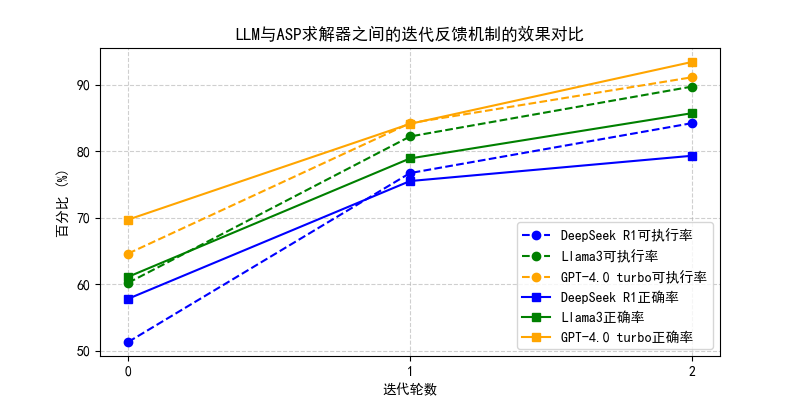
\includegraphics[width=\textwidth]{ablation.png}
    \caption{LLM与ASP求解器之间的迭代反馈机制的效果对比}
    \label{fig:ablation}
\end{figure}

\section{本章小结}